% Do not modify these
\documentclass[fleqn,10pt]{wlscirep}
\usepackage[utf8]{inputenc}
\usepackage[T1]{fontenc}



% -- Insert any custom LaTeX packages here --

% \package{natbib} % <-- Required for the Chicago citation style
% \package{apacite} % <-- Required for the APA citation style
% If you decide to use one of the styles above, remember to change the \bibliographystyle{} at the bottom of the document too!

\usepackage{listings} % <-- Required if you want to display program source code in your paper.


% -- End of custom LaTeX packages --


% Fill in your title
\title{Assignment Title}

% Do not modify the author tag below, just let it be blank
\author{}

% Fill in assignment abstract
\begin{abstract}
Lorem ipsum dolor sit amet, malorum numquam eum ei. Fierent argumentum persequeris ei vis, an cum adhuc consul mnesarchum. Id mel vidisse platonem intellegebat, ocurreret temporibus nam ei. No cum rebum iisque, ne aeterno deserunt electram eos. Te option euripidis intellegam eam, vix ad tempor labore discere.FDDFD
\end{abstract}


% Do not modify the following two lines
\begin{document}
% define the infrastructure
\ExplSyntaxOn
\keys_define:nn { coverpage }
 {
  assignment_title .tl_set:N 	= \hk_variable_assignment_title_tl,
  student_name  .tl_set:N 		= \hk_variable_student_name_tl,
  student_number     .tl_set:N 	= \hk_variable_student_number_tl,
  course_name .tl_set:N 			= \hk_variable_course_name_tl,
  course_code .tl_set:N			= \hk_variable_course_code_tl,
  due_date .tl_set:N 			= \hk_variable_due_date_tl,
  master_of .tl_set:N 			= \hk_variable_master_of_tl,
  group_size .tl_set:N 			= \hk_variable_group_size_tl,
 }
\cs_new_protected:Nn \use_coverpage:n
 {
  \keys_set:nn { coverpage } { #1 }
  \coverpage
 }
\cs_set_eq:NN \makecoverpage \use_coverpage:n
\cs_new:Nn \use_variable:n
 {
  \tl_use:c { hk_variable_#1_tl }
 }
\cs_set_eq:NN \use \use_variable:n
\ExplSyntaxOff



% Command for making the cover page

\newcommand{\coverpage}{%
\begin{titlepage}
\begin{center}
\begin{figure}[ht]
\centering

\includegraphics[width=0.5\linewidth]{images/hk-logo.pdf}
\end{figure}
\huge{Course Assignment}\\
\LARGE{Master of \use{master_of}}\\
\Large{Department of Technology}\\

\vskip10pt%
\begin{table}[ht]
\centering
\Large
\setlength{\tabcolsep}{0.5em}
\setlength\extrarowheight{1.2em}
\begin{tabularx}{0.8\linewidth}{lX}
\toprule
 Assignment title 	& \use{assignment_title} \\ \hline
 Course code 		& \use{course_code} \\ \hline
 Course name 		& \use{course_name} \\ \hline
 Due date			& \use{due_date} \\
 \bottomrule
\end{tabularx}%
\end{table}

\vskip10pt
\textbf{\Large{Declaration:}}\\

\if\use{group_size}1
Through the submission of this assignment, I hereby declare\\ that this report is the result of my own work, and that all\\ sources have been properly cited to throughout the text.
\vskip10pt%
\begin{table}[ht]
\centering
\Large
\setlength{\tabcolsep}{0.5em}
\setlength\extrarowheight{1em}
\begin{tabularx}{0.8\linewidth}{lX}
\toprule
 Student name 		& \use{student_name} \\ \hline
 Student ID number 	& \use{student_number} \\ 
 \bottomrule
\end{tabularx}%
\end{table}

\else 

Through the submission of this assignment, we hereby declare\\ that this report is the result of our own work, and that all\\ sources have been properly cited to throughout the text.
\begin{table}[ht]
\centering
\Large
\setlength{\tabcolsep}{0.5em}
\setlength\extrarowheight{1em}
\begin{tabularx}{0.8\linewidth}{lX}
\toprule
 Names of students 		& \use{student_name} \\ \hline
 Student ID numbers 	& \use{student_number} \\ 
 \bottomrule
\end{tabularx}%
\end{table}
\fi




\end{center}
\end{titlepage}
}


% Insert data for the hand-in's cover page
\makecoverpage{
	master_of 		 = \par{Fill in},  % Use either: Applied Computer Science | Human-Computer Interaction
	assignment_title = \par{Fill in},  % Title of your assignment
	course_code    	 = \par{Fill in},  % Course code (ex. MA110)
	course_name      = \par{Fill in},  % Course name (ex. Systems Development)
	due_date		 = \par{Fill in},  % Due date
	student_name     = \par{Fill in},  % Your name (or names, if group – separate names with ; semicolon)
	student_number   = \par{Fill in},  % Your student ID number (or numbers, if group – separate ID numbers with ; semicolon)
	group_size		 = 1, % Number of group members (used for the declaration text)
}


% Do not modify the following two lines
\flushbottom
\maketitle


% --INTRODUCTION--
\section{Introduction}
Insert your introduction here.
fefe XD XD XD 
% --RELATED WORK--
\section{Related Work}
Present related work here. 
You should read \cite{Webster2002-pw} on presenting a literature review.
Both journal papers and conference papers, such as \cite{Dingsoyr2014-xt}, are great sources.

\subsection{A subsection}
This is an example of a sub-section.

% --RESEARCH METHOD--
\section{Research Method}
Present your research method and/or design here. 
In \cite{Hevner2010-yw}, the authors discuss design science research.

Sometimes, you need to use code to illustrate your technical implementations.
Using \texttt{lstlisting} can help you with that:

\begin{lstlisting}[caption=Displaying Hello World in JavaScript]
console.log("Hello World!");
\end{lstlisting}


You might also want to display a formula, equation, stats, or other types of information requiring a math "mode" in \LaTeX.

% In-line using dollar signs
$E=mc^2$

% A free-standing formula with caption
\begin{figure}[h]
\[ E = m c^2 \]
\caption{Mass-energy equivalence}
\end{figure}

% --FINDINGS/RESULTS--
\section{Findings/Results}
Present your findings/results! 
It may be in the form of a table, such as in the case of Table \ref{tab:example}.
Upload data to Github \cite{Github_undated-kr}.

\begin{table}[ht]
\centering
\begin{tabular}{|l|l|l|}
\hline
\textbf{Condition} & \textbf{n} & \textbf{p} \\
\hline
A & 5 & 0.1 \\
A & 5 & 0.1 \\
\hline
\end{tabular}
\caption{Table caption}
\end{table}

% --DISCUSSION--
\section{Discussion}
A discussion of your findings, results and previous research goes here, perhaps with a reference to Figure \ref{fig:figure_label}.

\begin{figure}[!h]
\centering
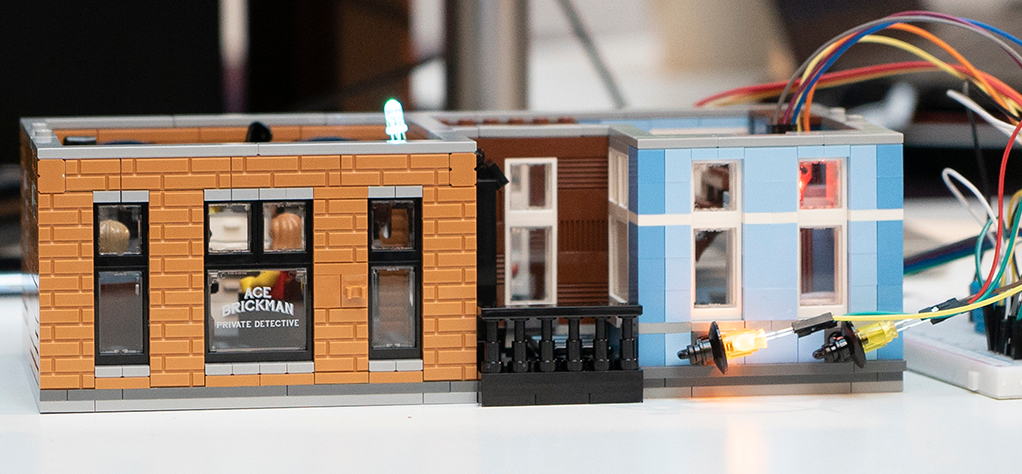
\includegraphics[width=0.5\linewidth]{images/sample_image.png}
\caption{Image caption}
\label{fig:figure_label}
\end{figure}

% --CONCLUSION--
\section{Conclusion}
Briefly conclude your study, and present thoughts on implications and further work.

\begin{itemize}
	\item One idea on further work;
	\item A second idea as well;
\end{itemize}

% --REFERENCES--
\bibliography{references} % <-- This line will generate the bibliography list automatically
\bibliographystyle{IEEEtran} % <-- Change this line if you want to use a different citation style

% Do not modify this last lines
\end{document}